\documentclass[tikz,border=8pt]{standalone}

\usepackage[utf8]{inputenc}
\usepackage[T1]{fontenc}
\usepackage{lmodern}
\usepackage{xcolor}
\usetikzlibrary{arrows.meta,calc,positioning}
\renewcommand{\familydefault}{\sfdefault}

\definecolor{medPurple}{HTML}{9B456F}
\definecolor{medBlue}{HTML}{249DC4}
\definecolor{latentGray}{HTML}{5A5A5A}
\definecolor{lossYellow}{HTML}{F1D897}
\definecolor{taskGreen}{HTML}{6EB79B}
\definecolor{panelGray}{HTML}{CFCFCF}
\definecolor{jepaOrange}{HTML}{E8893A}
\definecolor{removeRed}{HTML}{B50000}
\definecolor{patchGray}{HTML}{B7B7B7}

\tikzset{
  font=\sffamily,
  arrow/.style={-{Latex[length=2.0mm,width=1.7mm]}, draw=black, line width=1.1pt},
  dotarrow/.style={-{Latex[length=2.0mm,width=1.7mm]}, draw=black!60, dotted, line width=1.25pt},
  backarrow/.style={-{Latex[length=2.0mm,width=1.6mm]}, draw=jepaOrange!90!black, dashed, line width=1.05pt},
  panel/.style={rounded corners=8pt, draw=panelGray, dashed, line width=1.35pt, fill=white},
  image/.style={rectangle, draw=black, line width=0.75pt, fill=black!18, minimum width=2.1cm, minimum height=1.25cm, align=center, inner xsep=5pt, inner ysep=4pt, font=\bfseries\small},
  model/.style={rectangle, rounded corners=2pt, draw=none, fill=medPurple, text=white, minimum width=1.75cm, minimum height=1.02cm, align=center, inner xsep=6pt, inner ysep=4pt, font=\bfseries\small},
  frozen/.style={rectangle, rounded corners=2pt, draw=none, fill=medBlue, text=white, minimum width=1.75cm, minimum height=1.02cm, align=center, inner xsep=6pt, inner ysep=4pt, font=\bfseries\small},
  latent/.style={rectangle, draw=none, fill=latentGray, text=white, minimum width=1.75cm, minimum height=0.84cm, align=center, inner xsep=6pt, inner ysep=4pt, font=\bfseries\small},
  predictor/.style={rectangle, rounded corners=2pt, draw=none, fill=jepaOrange, text=white, minimum width=2.3cm, minimum height=0.92cm, align=center, inner xsep=7pt, inner ysep=4pt, font=\bfseries\small},
  loss/.style={rectangle, draw=none, fill=lossYellow, minimum width=3.7cm, minimum height=0.45cm, align=center, inner xsep=6pt, inner ysep=3pt, font=\bfseries\scriptsize},
  task/.style={rectangle, rounded corners=2pt, draw=none, fill=taskGreen, text=white, minimum width=3.25cm, minimum height=0.92cm, align=center, inner xsep=8pt, inner ysep=4pt, font=\bfseries\small},
  detail/.style={rectangle, rounded corners=2pt, draw=black!35, line width=0.5pt, fill=white, minimum width=2.35cm, minimum height=0.82cm, align=center, inner xsep=6pt, inner ysep=4pt, font=\bfseries\small},
  title/.style={font=\sffamily\bfseries\Large, align=center},
  panelLetter/.style={font=\sffamily\bfseries\LARGE},
  smallLabel/.style={font=\sffamily\scriptsize},
  flowLabel/.style={font=\sffamily\scriptsize, inner sep=1.4pt},
  redNote/.style={font=\sffamily\bfseries\small, text=removeRed}
}

\begin{document}
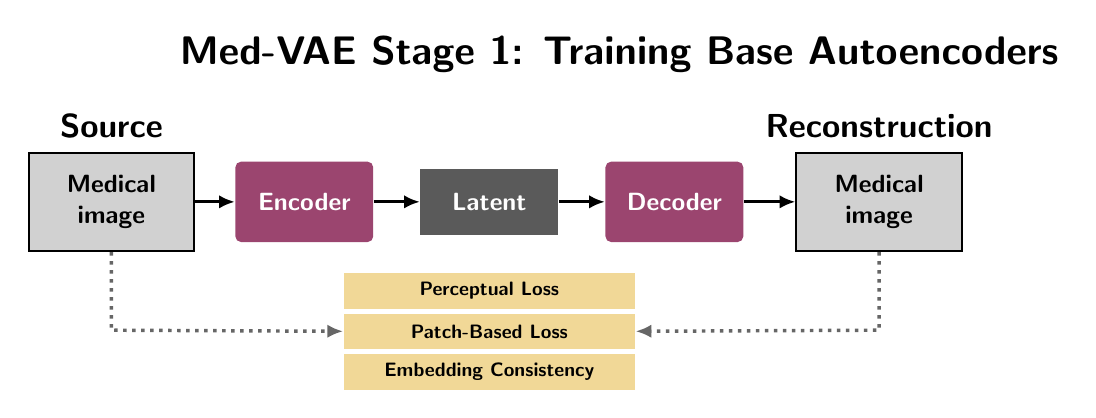
\begin{tikzpicture}[x=1cm,y=1cm]

% --------------------------------------------------------------------------
% Panel a — Med-VAE Stage 1: Training Base Autoencoders
% --------------------------------------------------------------------------
\node[title] at (9.3,4.52) {Med-VAE Stage 1: Training Base Autoencoders};

\node[font=\sffamily\bfseries\large] at (2.85,3.62) {Source};
\node[image] (aSrc) at (2.85,2.65) {Medical\\image};
\node[model] (aEnc) at (5.3,2.65) {Encoder};
\node[latent] (aLat) at (7.65,2.65) {Latent};
\node[model] (aDec) at (10.0,2.65) {Decoder};
\node[font=\sffamily\bfseries\large] at (12.6,3.62) {Reconstruction};
\node[image] (aRec) at (12.6,2.65) {Medical\\image};

\draw[arrow] (aSrc.east) -- (aEnc.west);
\draw[arrow] (aEnc.east) -- (aLat.west);
\draw[arrow] (aLat.east) -- (aDec.west);
\draw[arrow] (aDec.east) -- (aRec.west);

\node[loss] (aLoss1) at (7.65,1.52) {Perceptual Loss};
\node[loss, below=0.05cm of aLoss1] (aLoss2) {Patch-Based Loss};
\node[loss, below=0.05cm of aLoss2] (aLoss3) {Embedding Consistency};
\coordinate (aSrcDrop) at (2.85,1.02);
\coordinate (aRecDrop) at (12.6,1.02);
\draw[dotarrow] (aSrc.south) -- (aSrcDrop) -- (aLoss2.west);
\draw[dotarrow] (aRec.south) -- (aRecDrop) -- (aLoss2.east);

\end{tikzpicture}
\end{document}
